%% Select the report mode on (the default mode)
% See the documentation for more information about the available class options
% If you give option 'draft' or 'draft*', the draft mode is set on
\documentclass[report,draft*]{aaltoseries}
\usepackage[utf8]{inputenc}
\usepackage{booktabs}
\usepackage{adjustbox}
\usepackage{makecell}
\renewcommand\thesection{\arabic{section}}
% Lipsum package generates bullshit
\usepackage{lipsum,amsmath}
% Uncomment and give the correct language option if you are not writing in English
%\usepackage[<language>]{babel}
% The authors of the report
\author{Kunal Ghosh, 546247, Kunal.Ghosh@aalto.fi\\ Jussi K Ojala, 544605, Jussi.K.Ojala@aalto.fi \\Preeti Lahoti, 546878, Preethi.Lahoti@aalto.fi \\Shishir Bhattarai, 545688, Shishir.Bhattarai@aalto.fi}

% The title of the report
\title{ME-E4400 - Information Retrieval \\\\ Task 2: Recommender Systems}


\begin{document}
%% The abstract of the report
% Use this command!
%\draftabstract{Hello this is the draft abstract}
% If you want to include another abstract for the draft in another language,
% uncomment and give the language name as the optional argument
%\draftabstract[<language>]{\lipsum[4-6]}

%% Preface
% If you write this somewhere else than in Helsinki, use the optional location.
%\begin{preface}%[Optional location (if not defined, Helsinki)]
%\lipsum[1-4]
%\end{preface}
\let\cleardoublepage\clearpage
%% Table of contents of the whole report
\tableofcontents

%% The main matter, one can obviously use \input or \include
%\chapter{Recommender Systems}
\clearpage
\section{Introduction}
The goal of this project is to understand the basic concepts and methods of Information Retrieval, and analyze the performance of selected set of search technique combinations. The set of test documents was collected from the ACM digital library database. For each document, the collection includes the Title, Abstract and a Boolean \{0,1\} Relevance of the document with respect to the information need. \\
We focused on documents related to search task 2, which included 200 documents of which 114 were relevant under the studied information need "Recommender system" . \\
For this exercise, we chose eight different combinations of search techniques. Combinations were formed from different Stemmer, Stop word preprocessing and Similarity (Each combination is called a "Configuration" hence forth and in the accompanying software). Ranking methods used VSM with TF-IDF weights and BM25 e.g. \cite{Manning08}  as Similarity measures. Moreover we also studied the effect of morphological analysis with and with-out Stop Words using English Stemmer and English min Stemmer \cite{Porter80}, \cite{Porter01}, \cite{Krovetz93}. We also implemented and experiment with, Porter and K-Stemmer, but we selected the Stemmers that gave clearly different results for this report.

\paragraph{}
The report is organized as follows: Section 2 presents details of used Search Techniques, in Section 3 the statistics used for analysis are briefly introduced and in section 4 we discuss Results and in 5 summarize conclusions. Section 6 introduce our working method in this study.

%\chapterauthor{John Doe}

\section{Search techniques}
In this section we briefly describe our initial selection of different search techniques. These methods are combination of Similarities, Stemming and removal of stop words. As mentioned before, these combinations are referred to as "Configuration" in the accompanying software. 
\subsection{Similarities}
\subsubsection{BM25}
BM25 is the probabilistic Information Retrieval algorithm which uses bag of words retrieval function to rank the matching documents based on the query terms appearing in each document.\\
For given query $Q$ containing keywords $q_1, q_2, q_3 ... q_n$, the BM25 score of the document is given by,\\

\begin{equation}
score(Q,D) = \sum_{j=1}^{n}{IDF(q_i)\frac{f(q_i,D) \cdot (k_i+1)}{f(q_i,D)+K_1 \cdot (1-b+b \cdot \frac{\Vert D \Vert}{\text{avgdl}})}}
\end{equation}

where $f(q_i, D)$ is $q_i$'s term frequency in the document D, $\Vert D \Vert$ is the length of the document D in words, and \textit{avgdl} is average document length in text collection from which documents are drawn. $K_1$ and $b$ are free parameter $K_1 \in [1.2, 2.0]$ and $b \in [0, 1.0]$ \cite{Manning08}, for this study we selected default parameters $(b,K_1)=(0.75,1.2)$. IDF$(q_i)$ is defined
\begin{equation}
IDF(q_i) = \frac{N - n(q_i) + 0.5}{n(q_i) + 0.5}
\end{equation}

\subsubsection{TF-IDF}
TF-IDF is default weighting scheme for vector space models (VSM). In this document the TF-IDF refers to whole VSM not only the weights. The weights are defined as a product of the term frequency and inverse document frequency. There are couple different variants to define TF-IDF and the definition can vary for query and the document. Commonly term $t$ and document $d$ defines the TF-IDF as \\
\begin{equation}
W_{t,d} = (1 + \log(tf_{t,d})). \log\frac{N}{df_t}
\end{equation}
where $tf(t,d)$ is term frequency i.e. count of term $t$ in document $d$ and $df_t$ is number of document where term $t$ occurs.
In used vector model the documents are ranked on the basis of the cosine similarity between query and the document vectors. \\
\begin{equation}
sim(\vec{q}, \vec{d}) = cos(\vec{q}, \vec{d}) = \frac{\vec{q}\dot{}\vec{d}}	{\Vert 	\vec{q} \Vert \Vert \vec{d}}
\end{equation}		
\subsubsection{B25 vs TF-IDF}
We observe that both TF-IDF and BM25 use inverse document frequency to identify common words and rare words, and Term Frequency to give more weight to search terms appearing more frequently in the documents. However, BM25 applies an upper limit on the term frequency weights whereas TF-IDF do not. The result is that, for very long documents, the sheer number of occurrences of stop words can make a difference. Moreover BM25 applies field wise normalization on the length of the document, which is not present in TF-IDF. Thus in the pre-processing step, if we do not remove stop words then TFIDF might perform worse than BM25. 
\\BM25 has two tune-able parameters, parameter $K_1$ controls how quickly an increase in term-frequency should result in its saturation and parameter $b$ controls the field-length normalization. We use the default values without trying to optimize them.

\subsection{Stemming}
Stemming is the process of finding the base word (root word) in a language by removing the common morphological and inflectional endings from the words. It helps in term normalization process in text analysis like information retrieval. e.g. Transforming the words, run, running, runs and ran to the stem word "run". 
\subsubsection{English Stemmer / Porter Stemmer}
English stemmer is update of the Porter stemmer. Porter stemmer \cite{Porter80} \cite{Porter01} removes the common morphological and inflecional endings from words in English.
\subsubsection{K-Stemmer}
K-stemmer \cite{Krovetz93} is a morphological analyzer that reduces morphological variants to a root form.  For example, 'elephants' stemmed to 'elephant', 'amplification' to 'amplify' and 'european' to 'europe'. K-stemmer tries to avoid conflating variants that have different meanings.  For example `memorial' is related to `memory', and `memorize' is also related to `memory', but reducing those variants to `memory' would also conflate `memorial' with `memorize'.
\subsubsection{English Minimalist Stemmer}
English Minimalist stemmer is the least aggressive stemmer which only removes plural words. Hence words and their inflected forms will not be treated as the same words.

\subsubsection{K-Stemmer vs Porter Stemmer vs English Minimalist Stemmer}
The primary advantage of K-stemmer over Porter stemmer is that it allows any word form to be conflated to any other word form. That is, it returns words instead of truncated word forms. In general, K-stemmer requires a word to be in the lexicon  before it will reduce one word form to another. If a variant is explicitly mentioned in the lexicon, it is assumed to be unrelated to the (presumed) root, and the conflation is not done. 

\begin{table}[ht!]
\centering
\caption{Comparision of various stemming methods}
\label{tblstem}
\begin{tabular}{@{}llll@{}}
\toprule
Original       & Porter    & K-Stem       & EngMinStem     \\ \midrule
recommenders   & recommend & recommend   & recommender    \\
recommendation & recommend & recommend   & recommendation \\
association    & associ    & association & association    \\ \bottomrule
\end{tabular}
\end{table}

\subsection{Stop Words}
Removing the stop-words which appear frequently in all the documents can reduce the processing and query time as well as improve the accuracy of the information retrieval system. We use a default set of stop-words provided in the Lucene library. 


\section{Collected statistics}
We base our analysis on a few different Precision and Recall statistics which are briefly described below.
\subsection{Interpolated 11-point Precision Recall values}
This measure assumes that all relevant documents for the search task, are retrieved by the studied search method (i.e. recall is 100 \% for the query, Configuration combination). The 11-point Precision Recall Values are defined at 11 different recall level from recall 0\% to 100\% in steps of 10\% ($0.0, 0.1,\cdots, 1.0$ in the plots). The interpolated precision at each recall level is defined to be the maximum precision observed after that recall level.        
\subsection{Average 11 point precision recall Values}
In this study we have different queries for the same "information need". For a given "information need" (and a Search Technique/Configuration) this statistic is calculated by averaging precision values from the "11-point Interpolated Precision-Recall" values of all queries, at each recall level.
\subsection{Mean Average Precision (MAP)}
This measure provides a single-figure measure of quality across recall levels, for all queries given a Search Technique (Configuration).  The average precision for query is calculated as a mean of precision at all relevant documents before the $k^{th}$ relevant document, where k is a free parameter. \\
If the set of relevant documents for an information need $q_j \in Q$ is  $\{d_1,
\ldots d_{m_j}\}$ and  $R_{jk}$ is the set of ranked retrieval results from the top result until you get to document $d_k$, then 
\begin{equation}
\operatorname{MAP}(Q) = \frac{1}{\vert Q \vert}\sum_{q=1}^{\vert Q \vert} \frac{1}{m_j}\sum_{k=1}^{m_j}\operatorname{Precision}(R_{jk}) \!
\end{equation}

\section{Result and Comparison}
\begin{figure}[ht!]
\centering
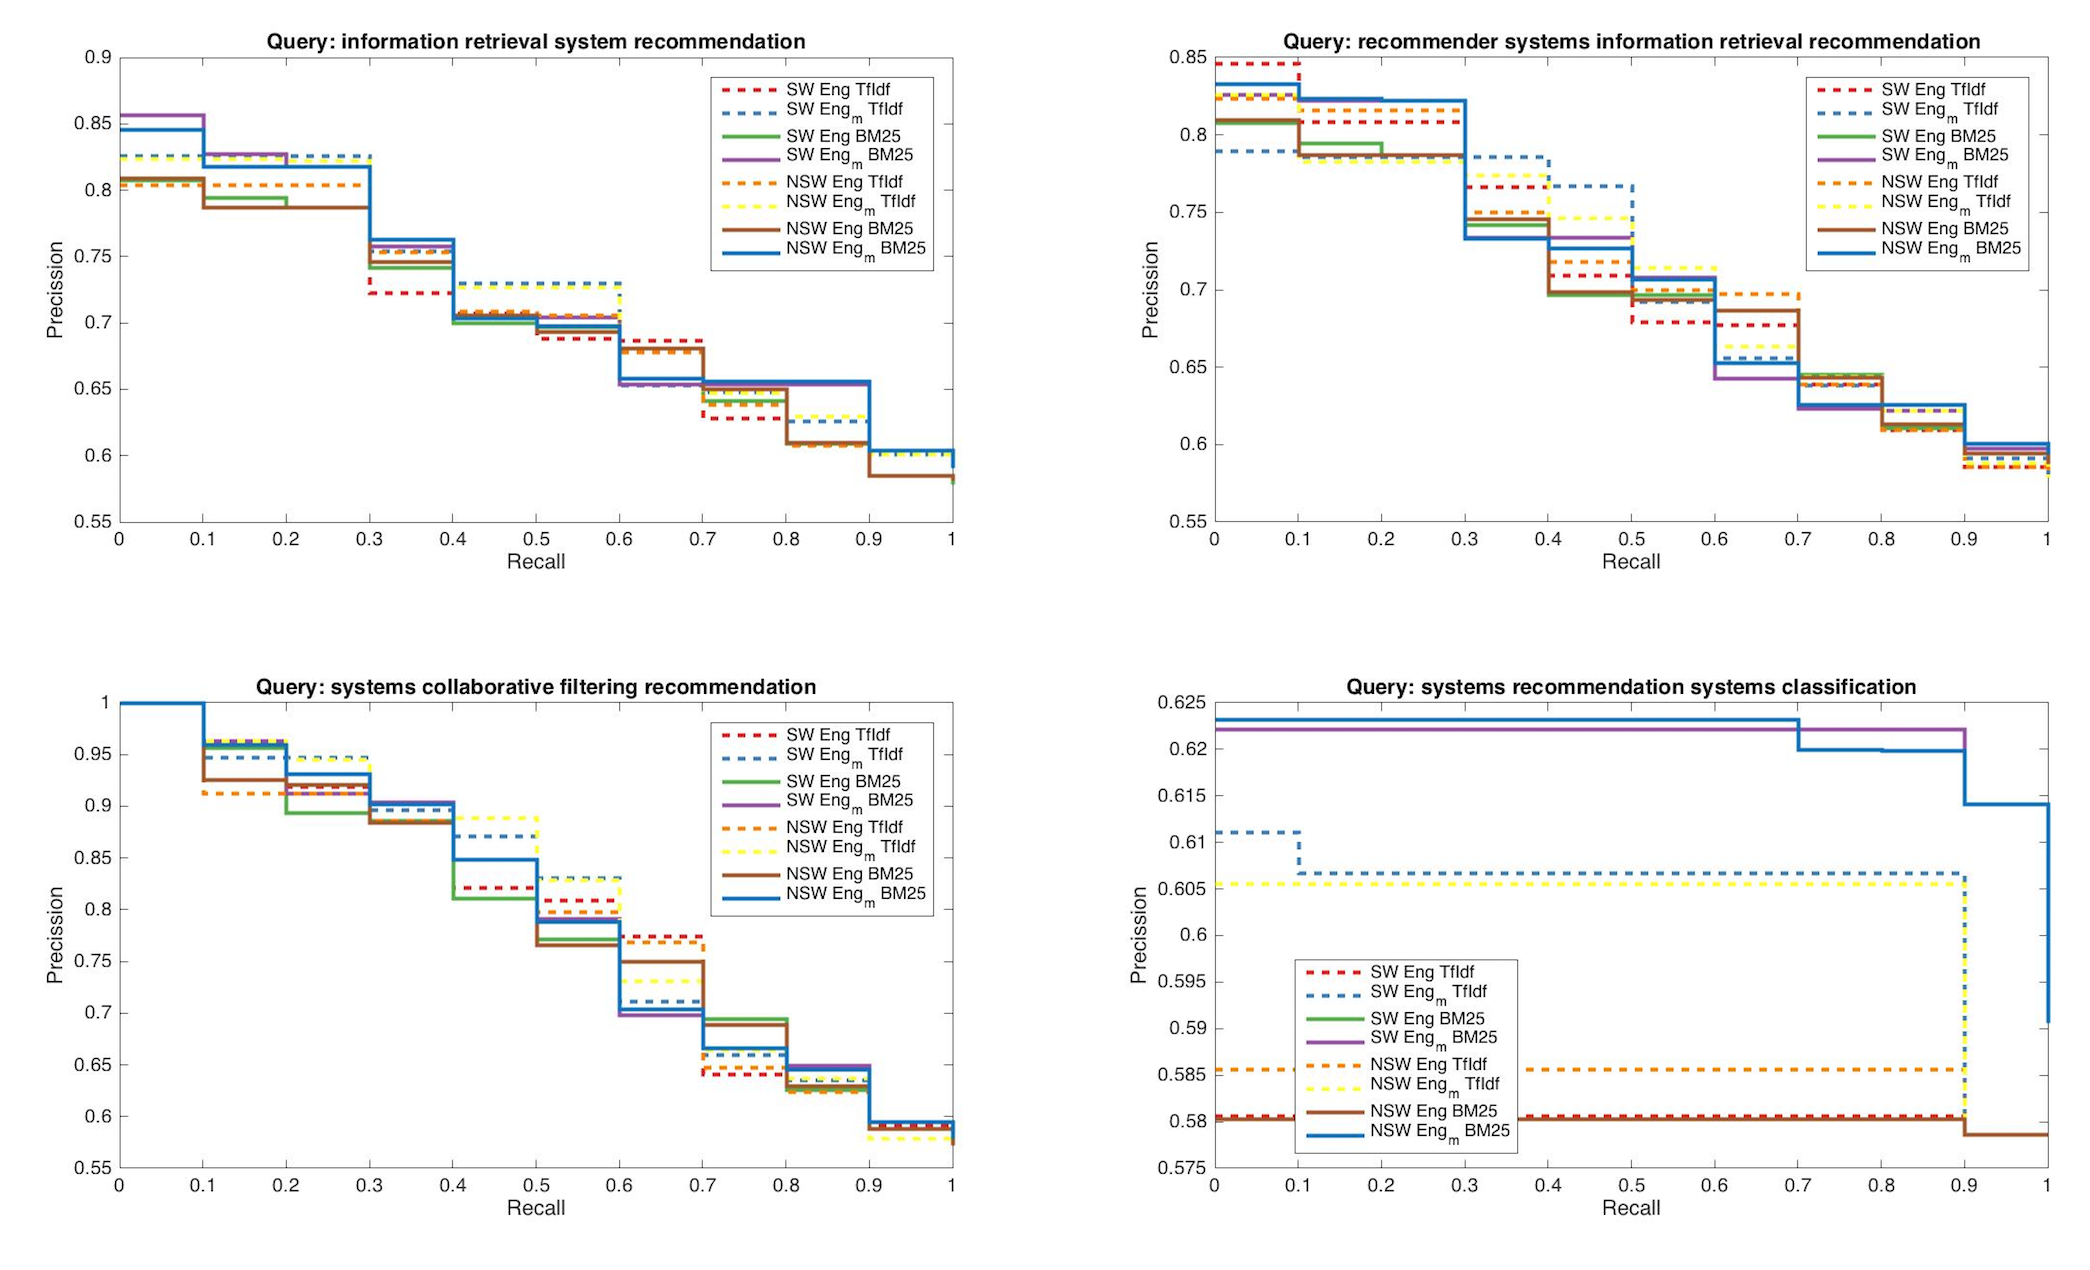
\includegraphics[width=\textwidth]{11PointPrecission.png}
\caption{ 11-point interpolated precision-recall curves with 8 search combination and four different queries (titles), SW = Stop Words Removed, NSW = Stop Words Not Removed}
\label{fig:1_1}
\end{figure} 

\begin{figure}[ht!]
\centering
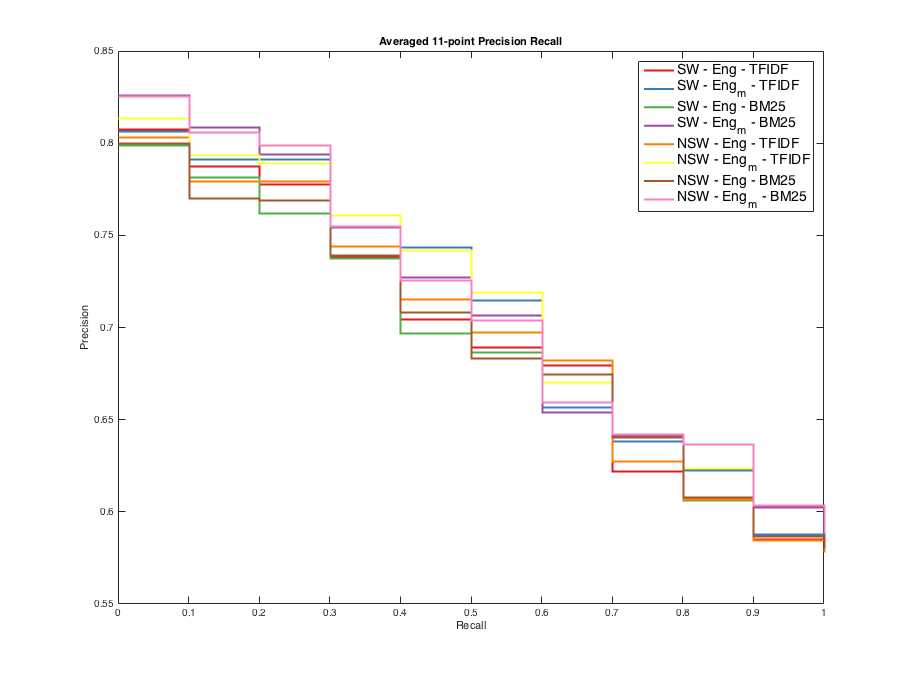
\includegraphics[width=\textwidth]{avg11point.png}
\caption{ 11-point average precision-recall curves with 8  search combination averaged over four different queries given in previous figure}
\label{fig:1_2}
\end{figure} 

\begin{figure}[ht!]
\centering
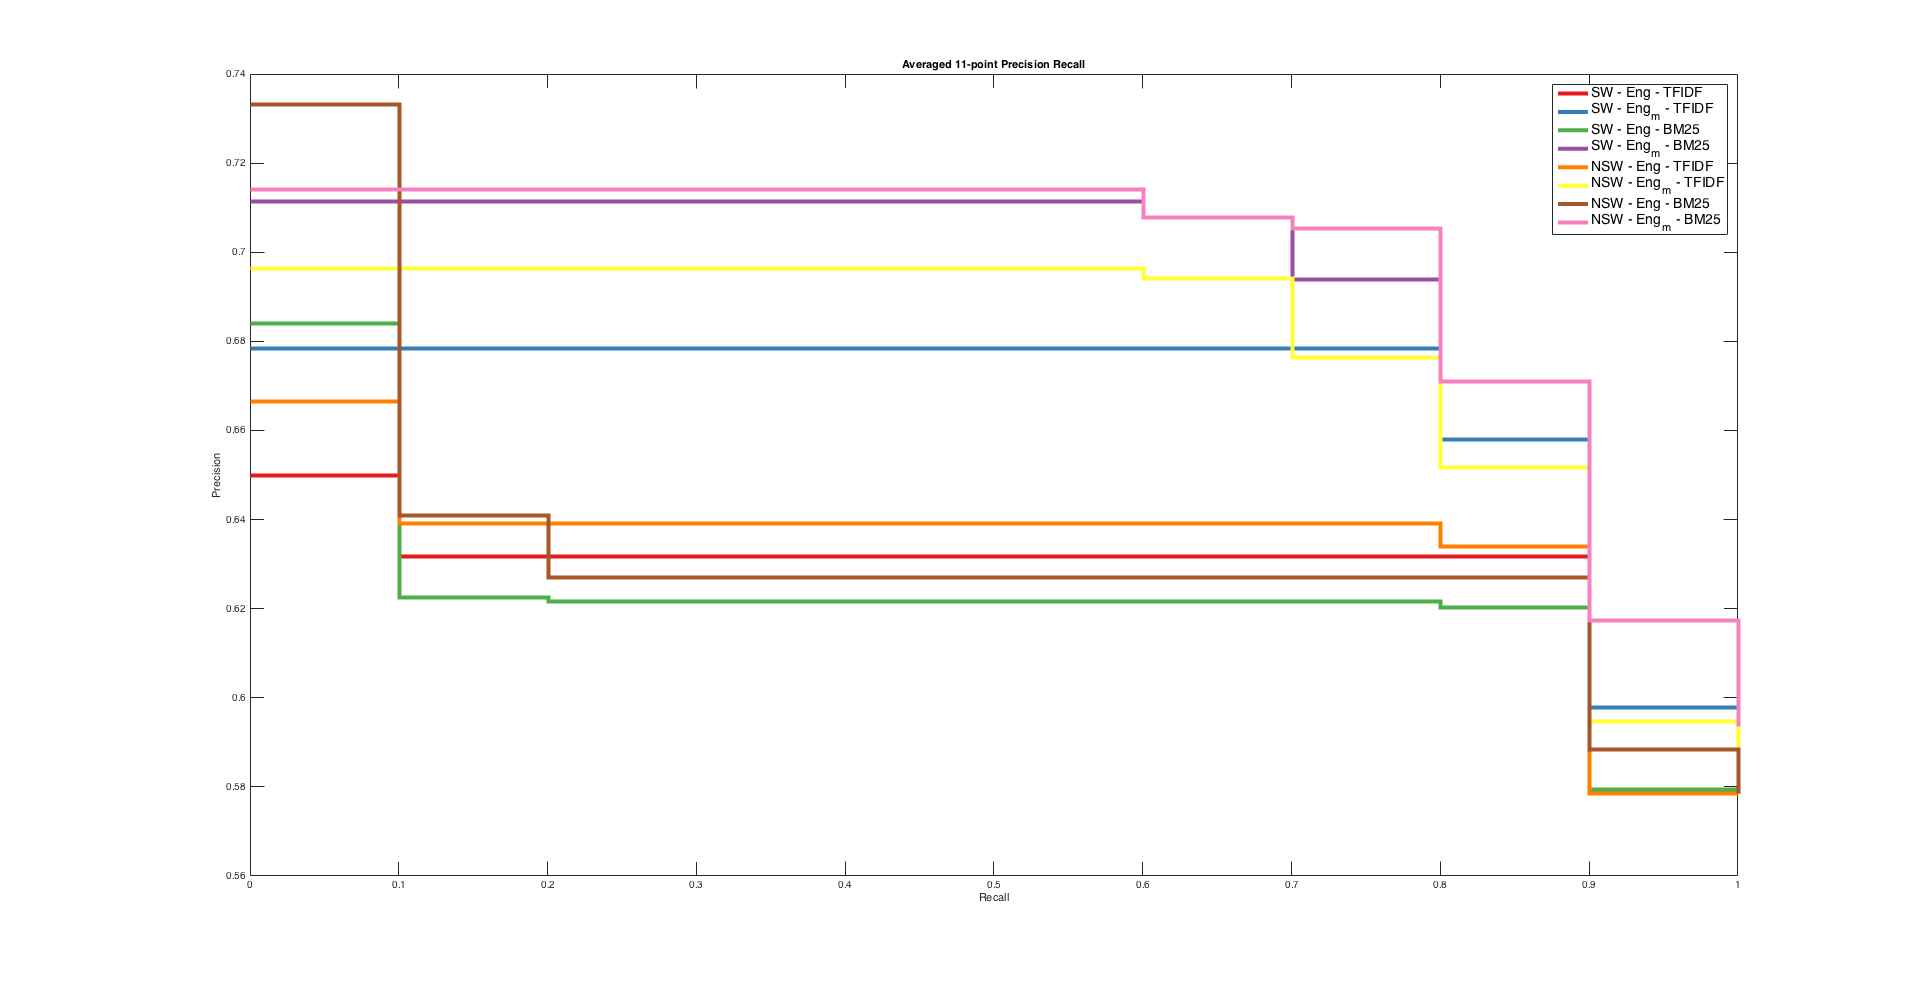
\includegraphics[scale=0.15]{recommendationSystems.png}
\caption{11-point precision recall values for the query "Recommendation System"}
\label{fig:recommendationSystem}
\end{figure}
Individual curves in plots shown in Figures \ref{fig:1_1} and \ref{fig:1_2} represent different search "configurations". From figure \ref{fig:1_2} we can see that the average performance of either algorithm BM25 and TFIDF does not depend on stop-word removal. In the plots pink and purple configuration differ only in stop word removal and give same precision value at given recall. More importantly their performance highly depends upon the used stemming algorithm. Pink curves represent BM25 with stop words and with English min stemmer and brown BM25,with stop words and English stemmer. Comparing these two curves we can see huge gap in top search results where pink is always higher than brown giving better results. For TFIDF we can see  yellow and orange curve, where yellow curve - english min stemmer  gives higher precision for same recall value than orange curve. - english stemmer. In this case also english min stemmer performs better than english stemmer.  \\It can be seen that the bottom right of figure \ref{fig:1_1} is significantly different from the others, in that, the precision values are lower and most of precision is achieved at high recall values. To explain this phenomenon we set a hypothesis that fewer "unique" terms in query might be the underlying cause. To examine this hypothesis, we plotted Figure (\ref{fig:recommendationSystem}) the 11-point precision recall curves for the query "Recommendation System" with only two terms.
The Figure \ref{fig:recommendationSystem} is quite similar to the one (bottom right) in figure \ref{fig:1_1}. This gives us a reason to believe that our hypothesis is correct. % Refer to this later %
On examining both of the above mentioned figures, we observed that for queries with fewer (3 or less) "unique" terms, BM25 performs better than TF-IDF. % Refer to this later %

\begin{table}[h!]
\centering
\caption{Mean Average Precision (MAP) @ K, across 5 queries. These are calculated over the first K relevant documents. SWR = Stop Words Removed, SWNR = Stop Words Not Removed, Eng\_m = English Minimal Stemmer, Eng = English Stemmer.}
\label{tblMAP}
\begin{tabular}{@{}lllll@{}}
\toprule
S.NO & Method                & MAP @ 5 & MAP @ 10 & MAP @ 20 \\ \midrule
1    & SWNR - Eng - BM25     & 0.676   & 0.692    & 0.694    \\
2    & SWNR - Eng\_m - BM25  & 0.771   & 0.761    & 0.736    \\
3    & SWNR - Eng - TFIDF    & 0.79    & 0.783    & 0.75     \\
4    & SWNR - Eng\_m - TFIDF & 0.845   & 0.807    & 0.764    \\
5    & SWR - Eng\_m - TFIDF  & 0.843   & 0.805    & 0.76     \\
6    & SWR - Eng - TFIDF     & 0.818   & 0.793    & 0.752    \\
7    & SWR - Eng - BM25      & 0.679   & 0.694    & 0.695    \\
8    & SWR - Eng\_m - BM25   & 0.786   & 0.765    & 0.741    \\ \bottomrule
\end{tabular}
\end{table}
We used the MAP to summarise our findings. From the Table \ref{tblMAP} we observed that, TF-IDF has higher MAP @ 5 and MAP @ 10 values. This means that on average TF-IDF would return more relevant documents among the top search results compared to BM25. This was averaged over queries with more than 3 unique terms.
\subsection{Anomalies in Document Collection}
To get further explanation for our results we looked at possible anomalies in our document set. We noticed that there were clearly longer abstracts in the document collection and took a look on search behavior of those documents. 
\begin{table}[]
\centering
\caption{Impact of document length on ranking methods}
\label{tbllength}
\adjustbox{max width = \textwidth}{
\begin{tabular}{@{}lllllll@{}}
\toprule
{S.No} & {Title} & \thead{ Length \\ of  document } & \thead{ Avg length \\ of document} &{ Relevance} & {TFIDF} & {BM25} \\ \midrule
{1} & \makecell{The European community and information technology}      & 2597             & 200                         & 0         & 104            & 88           \\
{2} & \makecell{Inconsistent Requirement: an Argumentation View}       & 2228              & 200                         & 1         & 141           & 163          \\
{3} & \makecell{Software fault tolerance in real-time embedded systems} & 833               & 200                         & 0         & 38            & 36           \\ 
{4} & \makecell{3PRS: a personalized popular program recommendation\\ system for digital TV for P2P social networks} & 166               & 200                         & 1         & 18            & 14           \\ 
{5} & \makecell{SVR-based music mood classification \\ and context-based music recommendations} & 118               & 200                         & 0         & 12            & 5           \\ 
{6} & \makecell{Social recommender systems} & 61               & 200                         & 1         & 6            & 13           \\ 
\bottomrule
\end{tabular}
}
\end{table}
Table \ref{tbllength} presents results for the query: "Information and recommendation systems classification" for configuration using English Stemmer and Stop Words removed. We wanted to understand whether the document size normalization works better in BM25, but the results indicate that there is not much difference between the two ranking methods. 

\section{Conclusion}
\begin{itemize}
\item The comparison of the different search combination is very case specific.
\item The results confirm obvious fact that query plays crucial role in determining how many relevant documents are retrieved in the top K results. 
\item Selection of correct stemmer has biggest impact on the results.  The less aggressive stemming of the document results in higher precision values across all recall values in this document collection.
\item BM25 performs better when the effective number of "unique" terms in the query is lower (3 terms or lower). However, the precision is still quite low and is achieved only after high recall levels are achieved.
\item On an average, TF-IDF returns much more relevant documents towards the beginning of the search results compared to BM25.
\item Removing stop words did not play any significant role. This feature could be more important when the document size grows and it can save space.

\end{itemize}
\section{Contributions}
The report writing and coding was done on a single computer with everyone pitching in with content, comments and suggestions. In such a mode of operation it is difficult to write individual contributions. It would be safe to assume that equal contributions were made by each team member.
% \item[11-point interpolated precision-recall curve]
% We analyzed 8 search combination with four different queries.



% We observe that data prepossessing is an important step in information retrieval tasks. Nature of stemming can have a significant impact on the retrieval of the documents. Aggresr.

\begin{thebibliography}{5}
%
\bibitem {Krovetz93}
"Viewing Morphology as an Inference Process", by Robert Krovetz, Proceedings of the ACM-SIGIR Conference on Research 
and Development in Information Retrieval, pp. 191-202, 1993
\bibitem {Porter80}
Porter, M. F. (1980). An algorithm for suffix stripping. Program: Electronic Library and Information Systems, 40(3), 211-218. 
\bibitem {Porter01}
Porter, M. F. (2001). Snowball: a language for stemming algorithms. Retrieved 26 January 2014 from http://snowball.tartarus.org/texts/introduction.html. (Archived by WebCite® at http://www.webcitation.org/6MmQJZdhV)
\bibitem{Manning08}
Manning, Christopher D., Prabhakar Raghavan, and Hinrich Schütze. Introduction to information retrieval. Vol. 1. No. 1. Cambridge: Cambridge university press, 2008.


\end{thebibliography}
\end{document}